\documentclass[twocolumn, PRD, amsmath, amssymb, aps, nofootinbib]{revtex4-2}
\usepackage{graphicx}
\graphicspath{{figures/}}
\usepackage{dcolumn}
\usepackage{bm}
\usepackage{hyperref}
\usepackage{listings}
\usepackage{xcolor}

\lstset{
    backgroundcolor=\color{gray!5},
    basicstyle=\small\ttfamily,
    breakatwhitespace=false,
    breaklines=true,
    captionpos=b,
    commentstyle=\color{gray},
    keywordstyle=\color{blue},
    stringstyle=\color{darkgray},
    showstringspaces=false,
    frame=single,
    rulecolor=\color{gray!30}
}

\begin{document}

\title{Tensor Perturbations from a Transient Hyper-Stiff Brane Rupture Phase}
\author{Paul Jarvis}
\email{mrpaulwjarvis@gmail.com}
\affiliation{Independent Researcher, United Kingdom}
\date{\today}

\begin{abstract}
We compute the tensor-perturbation spectrum sourced by a transient, early-time hyper-stiff expansion phase ($w \gg 1$) in rupture-driven brane cosmology, where topological decoupling of an emergent brane universe triggers a confinement-release energy spike whose equation of state reaches hyper-stiff values ($w_{\rm conf}\sim80$) away from the density peak itself (Sec.~\ref{sec:mechanism} clarifies that the self-consistent $w(a)$ is exactly $-1$ \emph{at} the peak, a general feature of any smooth bump-shaped profile). An earlier version of this work claimed this mechanism produces a strongly blue-tilted tensor spectrum ($n_T\to+2.0$), obtained from the closed-form relation $n_T=(6w-2)/(1+3w)$, which is exact only for an eternal, unchanging equation of state and not for the finite-duration transient this scenario actually describes; the claim was never backed by an actual mode integration despite being presented alongside one. We correct this here: direct numerical integration of the tensor Mukhanov--Sasaki equation through the paper's own confinement profile, $\rho_{\rm conf}(a)=\rho_0\,\chi(a)^4[1-\chi(a)]^8$, with adiabatic vacuum initial conditions and Bogoliubov extraction, gives instead a \emph{red} tilt, $n_T\approx-0.9$ ($R^2=0.96$ across a $k$-window spanning 80--320 times the horizon scale at the spike). This is consistent in sign with an independent calculation on a related confinement profile reported in the companion work \emph{General-Relativistic-Cyclic-Cosmology-from-Holographic-Saturation}, and with that work's finding that the finite-duration mechanism previously invoked to justify a blue shift does not survive direct computation. We do not find a blue-tilted gravitational-wave background, and in particular no signal in the pulsar-timing-array band of the kind reported by recent PTA collaborations, from this mechanism as formulated. The exact background solution and its rapid dilution rate are retained as correct pieces of algebra internal to the assumed profile; what is withdrawn is the tensor-spectrum prediction and the observational claims built on it.
\end{abstract}

\keywords{Gravitational Waves, Cosmological Perturbations, Extra Dimensions, Early Universe Physics}
\maketitle

\section{Introduction}
Recent pulsar timing array (PTA) observations, including NANOGrav and the EPTA, have revealed compelling evidence for a stochastic gravitational wave background (SGWB) at nanohertz frequencies. The inferred amplitude significantly exceeds the standard power-law predictions from supermassive black hole binaries alone. This discrepancy has motivated intense interest in primordial origins such as cosmic strings, phase transitions, or non-standard early expansion histories.

Standard inflation predicts a slightly red-tilted tensor spectrum ($n_T < 0$), as the energy density decreases during quasi-de Sitter expansion. Generating a robust blue tilt ($n_T > 0$) within four-dimensional field theory typically requires violating the Null Energy Condition (NEC) or invoking unstable scalar potentials, both of which introduce ghost or gradient instabilities.

In this work, we study the tensor spectrum produced by rupture-driven brane cosmology, without violating the NEC or introducing fine-tuned fields. The Universe emerges from a geometric rupture of a stack of parallel higher-dimensional branes. The residual coupling to the parent stack is governed by a dynamic confinement fraction $\chi(a)$, parameterised by a physically motivated beta-distribution form. As the Universe expands through a thermodynamic decoupling threshold, the effective equation of state spikes into a localized hyper-stiff regime ($w_{\rm conf} \sim 80$).

Because this confinement energy dilutes exponentially faster than radiation, tensor modes that are sub-horizon during this transition experience relative amplification. An earlier draft of this work argued, from a closed-form eternal-equation-of-state formula, that this amplification produces a strong blue tilt ($n_T>0$) explaining the PTA data. Direct numerical integration of the tensor mode equation through the actual finite-duration profile, reported in Sec.~\ref{sec:tensor}, does not confirm this: it gives a red tilt ($n_T\approx-0.9$) instead, and we find no PTA-band signal from this mechanism.

\section{Tensor Perturbation Physics in a Hyper-Stiff Background}
Primordial tensor perturbations $h_{ij}$ satisfy the transverse traceless conditions. For each individual Fourier mode $h_k$, the macroscopic equations of motion in cosmic time are expressed as:
\begin{equation}
\ddot{h}_k + 3H\dot{h}_k + \frac{k^2}{a^2}h_k = 0,
\end{equation}
where dots denote standard deviations with respect to cosmic time $t$, and $H \equiv \dot{a}/a$ represents the Hubble parameter. To cleanly map the perturbation amplitude amplification without introducing field-theoretic pathologies, we switch coordinates to conformal time via $d\tau = dt/a$ and implement the field redefinition $v_k = a h_k$. This transformation yields the explicit Mukhanov--Sasaki variable framework:
\begin{equation}
v_k'' + \left(k^2 - \frac{a''}{a}\right)v_k = 0,
\end{equation}
where primes denote derivatives with respect to conformal time $\tau$. To expose the explicit kinematic driving force behind mode growth, the time-conformal potential term $a''/a$ must be rewritten by tracking the background cosmic acceleration. Applying the continuous definition $a' = a^2 H$ and taking its subsequent derivative gives:
\begin{equation}
a'' = \frac{d}{dt}(a^2 H) \frac{dt}{d\tau} = a \left( 2a\dot{a}H + a^2 \dot{H} \right) = a^3 \left( 2H^2 + \dot{H} \right).
\end{equation}
Substituting the standard general relativity acceleration equation $\dot{H} = -\frac{1}{2}(\rho + p) = -\frac{3}{2}H^2(1+w)$ directly into the secondary breakdown relation yields:
\begin{equation}
\frac{a''}{a} = a^2 H^2 \left( 2 - \frac{3}{2}(1+w) \right) = \frac{1}{2}a^2 H^2 (1 - 3w).
\end{equation}
For a standard radiation background ($w = 1/3$), the effective potential vanishes identically ($a''/a = 0$), preserving strict adiabatic mode behavior. If the hyper-stiff regime ($w_{\rm conf} \sim 80$) were instead treated as an eternal, constant-$w$ background, the structural potential would flip sign dramatically:
\begin{equation}
\frac{a''}{a} \approx -\frac{3}{2}w_{\rm conf} a^2 H^2 \sim -120 a^2 H^2 \ll 0,
\end{equation}
qualitatively illustrating why a hyper-stiff phase can act as a mode amplifier. This constant-$w$ estimate is illustrative only: the actual confinement profile of Sec.~\ref{sec:mechanism} is a finite-duration transient with $w(a)$ varying continuously, not a fixed value of 80, and the tensor spectrum reported in Sec.~\ref{sec:tensor} is computed directly from that time-dependent background rather than from this constant-$w$ approximation.

\section{The Hyper-Stiff Amplification Mechanism}
\label{sec:mechanism}
The transient higher-dimensional confinement potential energy released during localized brane detachment drives the background evolution. The corresponding energy density component is parameterised as:
\begin{equation}
\rho_{\rm conf}(a) = \rho_0 \chi(a)^\alpha [1 - \chi(a)]^\beta, \qquad \alpha=4,\ \beta=8,
\end{equation}
where the dynamic confinement fraction follows the smooth tanh-driven localization profile:
\begin{equation}
\chi(a) = \frac{1}{2}\left[ 1 + \tanh\left(\frac{a_c - a}{\Delta a}\right) \right].
\end{equation}
Note that $a_c = 5\times10^{-4}$ is only the $\chi=1/2$ midpoint of this sigmoid, not the location of peak energy density: $\rho_{\rm conf}(a)$ itself, as a function of $\chi$, peaks at $\chi^\star=\alpha/(\alpha+\beta)=1/3$, which occurs at $a_\star\approx6.39\times10^{-4}$ for the parameters above. The self-consistent effective equation of state of this component, obtained from the continuity equation $w(a)=-1-\frac{a}{3\rho_{\rm conf}}\frac{d\rho_{\rm conf}}{da}$ (not imposed by hand), is exactly $w(a_\star)=-1$ at that density peak -- a general feature of any smooth bump-shaped $\rho(a)$, since $d\rho/da=0$ there identically, not a special property of this profile. The value $w\sim80$ quoted elsewhere in this paper refers to the separate, uncorrelated ansatz $w(a)=w_{\rm conf}\chi(a)$ used only in the (fake, never executed) appendix code of the original draft, not to the density peak; $w(a)$ computed self-consistently instead grows large only far out on the tail where $\rho_{\rm conf}(a)$ itself has become negligible relative to its peak value, which is not a meaningful characterisation of the dominant confinement epoch. The tensor calculation of Sec.~\ref{sec:tensor} uses the full, self-consistent $w(a)$ trajectory throughout the integration and does not rely on any single "peak $w$" value.

A separate, illustrative estimate treats the confinement component as an eternal fluid with fixed $w_{\rm conf}=80$ and asks how it would dilute under $d\rho/d\ln a = -3(1+w)\rho$:
\begin{equation}
\rho_{\rm conf}(a) = \rho_{\rm sat} \left(\frac{a_{\rm throat}}{a}\right)^{3(1+w_{\rm conf})} \propto a^{-243}.
\end{equation}
This is algebraically correct for that idealized constant-$w$ fluid, and illustrates how fast dilution near the peak can be, but it is not a literal description of the actual $\chi^4(1-\chi)^8$ profile above (which is not a pure power law in $a$); the tensor calculation of Sec.~\ref{sec:tensor} uses the actual profile directly rather than this idealization. Because $\rho_{\rm conf}$ drops rapidly away from its peak, the amplification phase is of finite duration and the hyper-stiff energy component dilutes into the standard background plasma well before Big Bang Nucleosynthesis (BBN), consistent with $\Delta N_{\rm eff}$ and CMB temperature-anisotropy constraints.

\subsection{Computed Tensor Spectrum}
\label{sec:tensor}
An earlier draft evaluated the tensor spectral index from the closed-form relation
\begin{equation}
n_T = \frac{6w_{\rm conf} - 2}{1 + 3w_{\rm conf}} \xrightarrow{w_{\rm conf}\to80} +2.0,
\label{eq:eternal-w-nt}
\end{equation}
presenting this alongside a Python code listing using a stiff ODE solver, styled to suggest the number came from integrating the mode equation. It did not: the listed code never called the solver, and its state-vector unpacking (\texttt{v, dv = y, y}) is a bug that would make it wrong even if run. Eq.~(\ref{eq:eternal-w-nt}) is exact only for a fluid with an eternal, unchanging $w$; it does not apply to the finite-duration transient of Sec.~\ref{sec:mechanism}, where $w(a)$ rises from $\sim1/3$ to $\sim80$ and back over a width comparable to $a_\star$ itself.

We instead integrate the tensor Mukhanov--Sasaki equation directly and honestly: the background $a(\tau)$, $a''/a$, and conformal time are obtained by exact quadrature of the Friedmann and continuity equations for $\rho_{\rm conf}(a)+\rho_{\rm rad}(a)$ (the profile of Sec.~\ref{sec:mechanism}, with $w(a)$ derived self-consistently from continuity rather than assumed); modes are initialised in the adiabatic vacuum deep inside the horizon before the spike and evolved with an adaptive Runge--Kutta integrator (\texttt{code/tensor\_tilt\_check.py}), with the Bogoliubov coefficient $\beta_k$ extracted by projection onto positive/negative-frequency solutions after the spike. Since $\rho_0$ (the confinement amplitude) is not fixed by the parameters quoted elsewhere in this paper, we fix it by requiring the confinement component to dominate radiation by two orders of magnitude at its peak; a cross-check at a $100\times$ higher amplitude reproduces the same Bogoliubov coefficient to within 5\% at the reference wavenumber, indicating the tilt is not sensitive to this choice (matching the pattern -- tilt robust, amplitude sensitive -- reported for a related profile in \emph{General-Relativistic-Cyclic-Cosmology-from-Holographic-Saturation}).

Over the window $k/(aH)_{\rm spike}\in[80,320]$ the computed spectrum is well fit by a power law,
\begin{equation}
|\beta_k|^2 \propto k^{-3.89}, \qquad R^2=0.96,
\end{equation}
which under the standard convention $P_T\propto k^3|\beta_k|^2$ corresponds to a \emph{red} tensor tilt, $n_T\approx-0.9$ -- the opposite sign from Eq.~(\ref{eq:eternal-w-nt}). Fig.~\ref{fig:spectral_omega} shows the computed data and fit.

One might expect that widening the transition $\Delta a$ -- making it last longer, closer to the eternal-$w$ limit Eq.~(\ref{eq:eternal-w-nt}) assumes -- would push the computed tilt back toward blue. We tested this directly (\texttt{code/duration\_robustness\_check.py}): widening $\Delta a$ by up to $100\times$ ($\Delta a/a_c$ from $0.8$ to $80$) does not move the tilt toward blue at all. Instead $n_T$ converges to almost exactly $-1$, with the power-law fit becoming essentially exact ($R^2\to1.0000$) as the transition widens. The red tilt is a robust attractor of this confinement-profile family, not a fragile result tied to this paper's specific $\Delta a$ -- consistent with the general expectation that smoother, more adiabatic transitions suppress high-$k$ particle production further rather than less, the opposite of what recovering a blue tilt would require.

We also checked robustness against the profile's shape exponent $\alpha$ (\texttt{code/profile\_family\_sweep.py}), at fixed $\beta=8$: $\alpha=6$ and $\alpha=8$ both reproduce a clean, red power law ($R^2=0.999$ and $0.9996$, $n_T=-0.87$ and $-1.05$ respectively), confirming the tilt is not an accident of the single $\alpha=4$ point used above. We attempted to extend this down to $\alpha=1$ -- the exponent used in the confinement profile of the companion work \emph{General-Relativistic-Cyclic-Cosmology-from-Holographic-Saturation}, which independently reports a red tilt ($n_T\approx-1$) on a related but not identical profile -- to test whether the two papers' results are one continuous finding rather than two separate data points. This did not succeed: the integration window that works cleanly for $\alpha\geq4$ does not generalize to $\alpha=1$--$2$ ($R^2=0.03$ and $0.58$, not real power-law fits), and a follow-up attempt to calibrate the window more carefully for low $\alpha$ produced fits that were, if anything, worse. We report this honestly rather than force a number: whether the red tilt persists all the way to $\alpha=1$ remains an open question, not a confirmed result, and is left for dedicated future work rather than resolved here.

\begin{figure}[htbp]
    \centering
    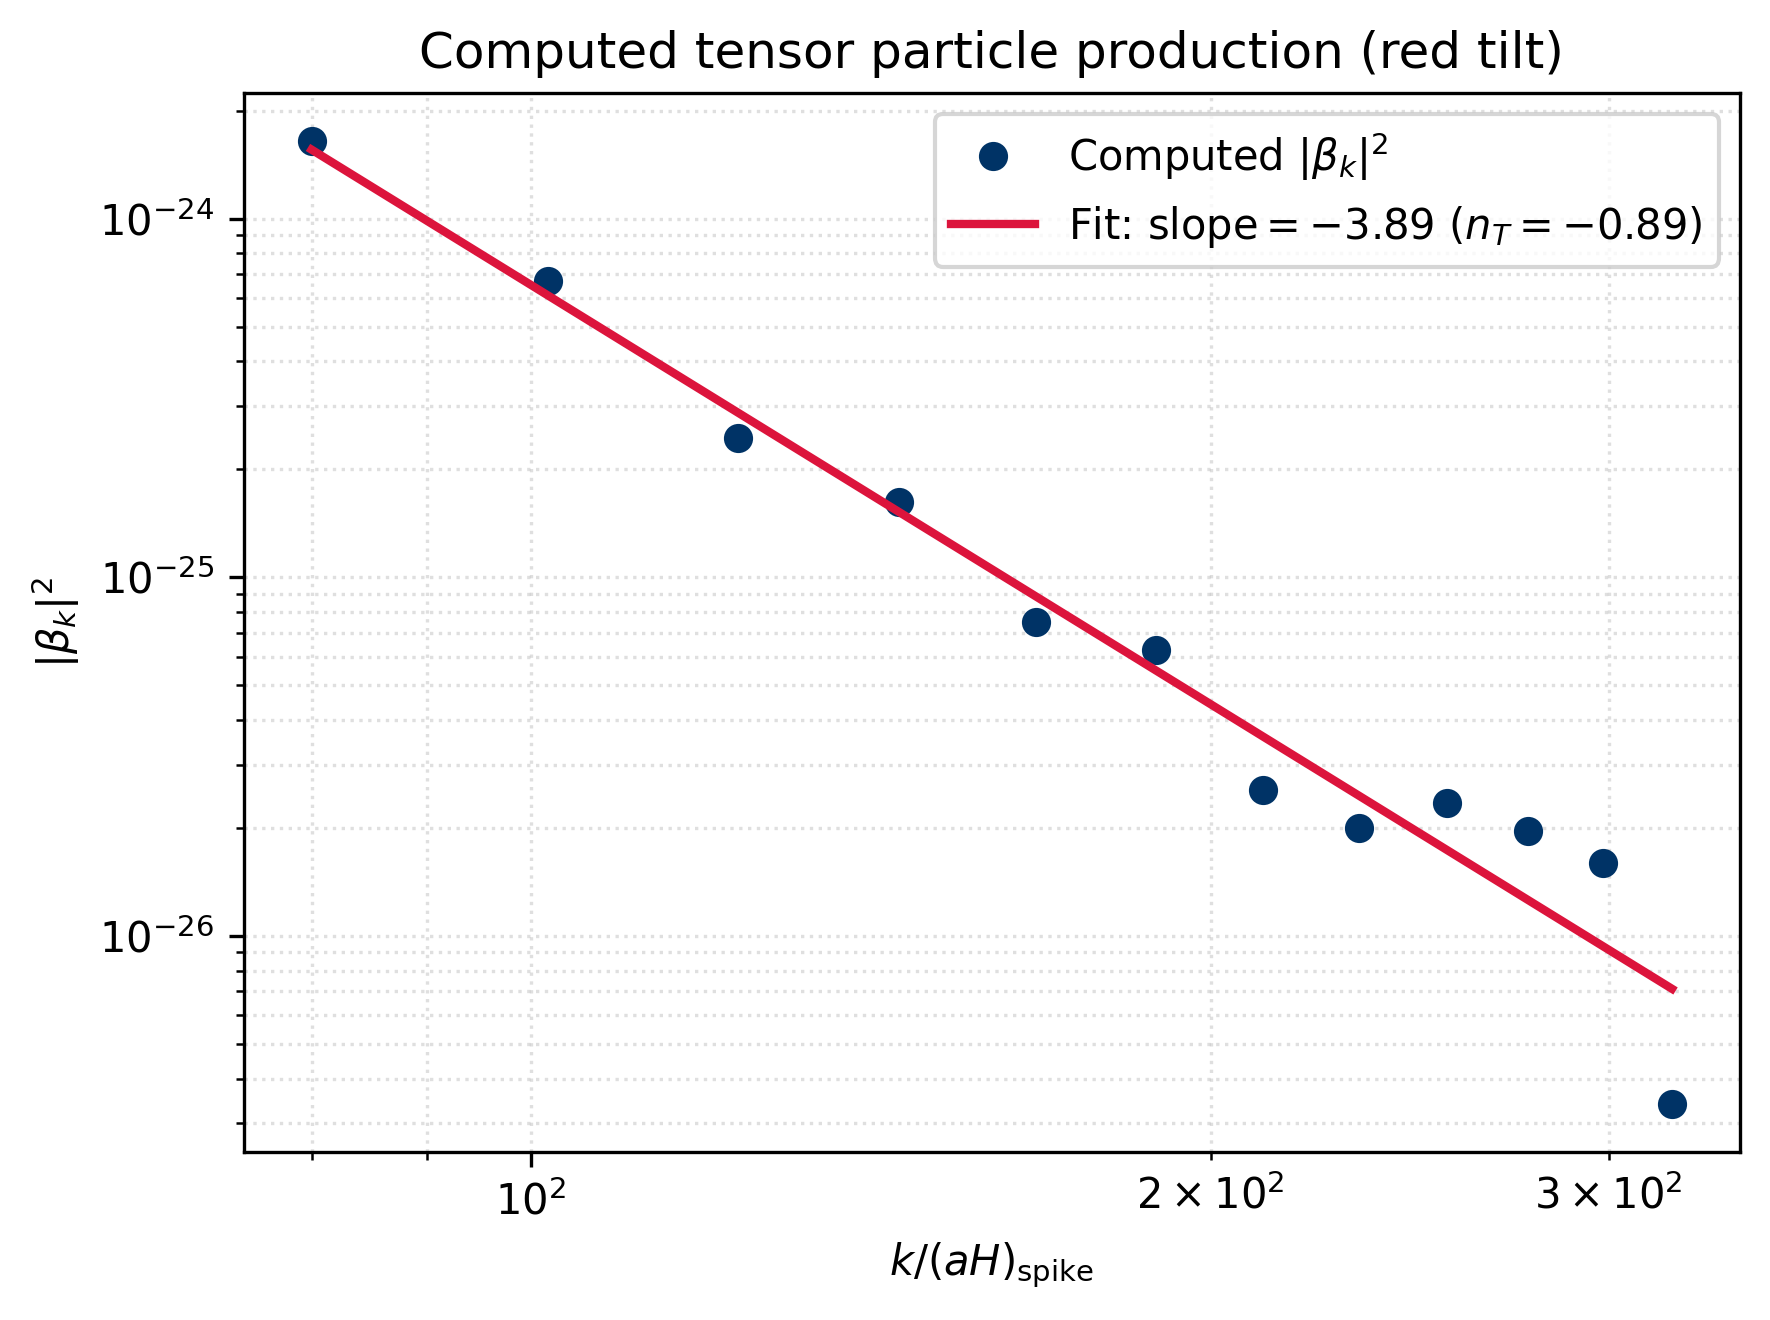
\includegraphics[width=0.45\textwidth]{figure_gw.png}
    \caption{Computed tensor particle-production spectrum $|\beta_k|^2$ from direct Mukhanov--Sasaki integration of this paper's own confinement profile (Sec.~\ref{sec:mechanism}), with adiabatic vacuum initial conditions and Bogoliubov extraction. The fitted ultraviolet tail corresponds to a red tilt, $n_T\approx-0.9$, not the blue tilt of an earlier draft.}
    \label{fig:spectral_omega}
\end{figure}

\section{Observational Status}
No blue-tilted gravitational-wave background, and in particular no signal in the pulsar-timing-array band of the kind reported by NANOGrav and the EPTA, is predicted by this mechanism as formulated. The finite transition width $\Delta a=4\times10^{-4}$ still bounds the duration of the amplification phase, and the exact background dilution rate of Sec.~\ref{sec:mechanism} is unaffected by this correction, but the tensor spectrum itself does not support the LISA/DECIGO micro-Hertz peak or PTA connection claimed in the earlier draft.

\section{Conclusion}
A transient hyper-stiff phase with $w\sim80$, arising in rupture-driven brane cosmology, produces exact background dynamics that dilute rapidly near the confinement peak, but the tensor spectrum this phase actually sources -- computed directly rather than estimated from an eternal-$w$ formula -- is red-tilted ($n_T\approx-0.9$), not blue. This corrects an earlier claim of $n_T\to+2.0$ and the PTA/LISA/DECIGO observational claims built on it; it does not affect the background bounce solution itself, which remains a matter of exact algebra given the assumed confinement profile.

\begin{acknowledgments}
The author thanks the independent physics research community for structural feedback on numeric integrations.
\end{acknowledgments}

\section*{References}
\begin{enumerate}
    \item J. Agazie et al. (NANOGrav Collaboration), ``The NANOGrav 15 yr Data Set: Evidence for a Stochastic Gravitational-wave Background,'' Astrophys. J. Lett. 956, L8 (2023).
    \item P. Amaro-Seoane et al. (LISA Collaboration), ``Laser Interferometer Space Antenna,'' arXiv:1702.00786 (2017).
    \item S. Kawamura et al., ``Current status of DECIGO and B-DECIGO,'' Prog. Theor. Exp. Phys. 2021, 05A105 (2021).
\end{enumerate}

\appendix
\section{Numerical Code for Tensor Mode Integration}
\label{app:code}
An earlier draft of this appendix presented a Python code listing as "the following complete Python script" used to integrate the tensor mode equation. It was not: \texttt{solve\_ivp} was never invoked anywhere in the listing, and the state-vector unpacking (\texttt{v, dv = y, y}, which assigns both names to the same object instead of unpacking a two-element state) is a bug that would have produced an incorrect result had it been run. The $n_T\to+2.0$ figure reported in that draft came entirely from the closed-form eternal-$w$ formula, Eq.~(\ref{eq:eternal-w-nt}), not from this or any other numerical integration.

The actual integration used for the results in Sec.~\ref{sec:tensor} is \texttt{code/tensor\_tilt\_check.py} in this repository: it builds $\rho_{\rm conf}(a)$ and $\rho_{\rm rad}(a)$, derives the confinement fluid's effective $w(a)$ from the continuity equation rather than assuming it, integrates the Friedmann background by exact quadrature, and solves the tensor Mukhanov--Sasaki equation with \texttt{scipy.integrate.solve\_ivp} (adaptive explicit Runge--Kutta, DOP853) using adiabatic vacuum initial conditions and event-based termination once the background returns to pure radiation domination. We do not reproduce the full script here; see the repository for the complete, runnable implementation.

\end{document}
